% -*- latex -*-
%%%%%%%%%%%%%%%%%%%%%%%%%%%%%%%%%%%%%%%%%%%%%%%%%%%%%%%%%%%%%%%%
%%%%
%%%% This TeX file is part of the course
%%%% Introduction to Scientific Programming in C++/Fortran2003
%%%% copyright 2017-9 Victor Eijkhout eijkhout@tacc.utexas.edu
%%%%
%%%% function.tex : functions
%%%%
%%%%%%%%%%%%%%%%%%%%%%%%%%%%%%%%%%%%%%%%%%%%%%%%%%%%%%%%%%%%%%%%

A~\indexterm{function}
(or~\emph{subprogram}\index{subprogram|see{function}}) is a way to
abbreviate a block of code and replace it by a single line.
This is foremost a code structuring device: by giving a function a
relevant name you introduce the terminology of your application into
your program.

\begin{itemize}
\item Find a block of code that has a clearly identifiable function.
\item Turn this into a function: the function definition will contain
  that block, plus a header and (maybe) a return statement.
\item The function definition is placed before the main program.
\item The function is called by its name.
\end{itemize}

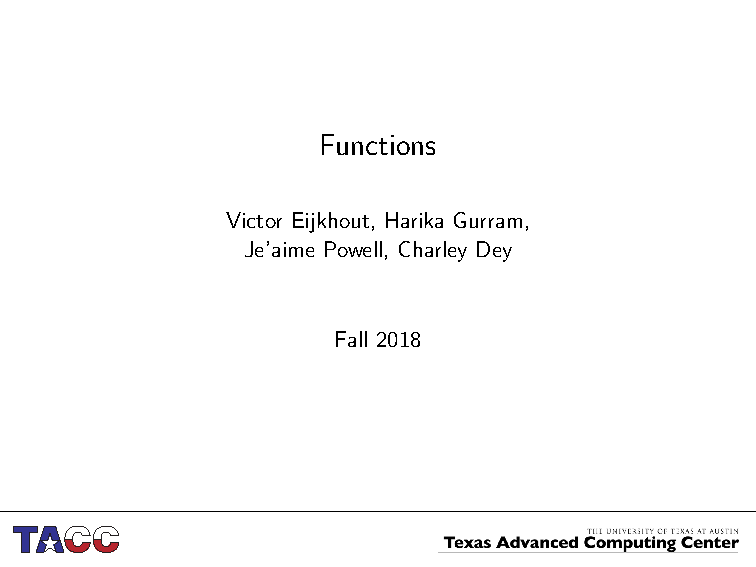
\includegraphics[scale=.5]{function}

\begin{slide}{Turn blocks of code into functions}
  \label{sl:function-intro}
  \begin{itemize}
  \item Code fragment with clear function:
  \item Turn into \emph{subprogram}: function \emph{definition}.
  \item Use by single line: function \emph{call}.
  \end{itemize}
\end{slide}

Using a function can also shorten your code, since it replaces two similar
code blocks with one function definition and two calls.

Even if the number of lines doesn't go down, there are still reasons
for using functions.
\begin{itemize}
\item By removing \indexterm{code duplication} you have removed a
  likely source of future errors: if you later edit one occurrence of
  the code block, you're likely to forget the other.
\item By introducting a function name you have introduced
  \indexterm{abstraction}: your program now uses terms related to your
  problem, and not only \lstinline{for} and \lstinline{int} and such.
\end{itemize}

\Level 0 {Function definition and call}

There are two sides to a function:
\begin{itemize}
\item
  The \indextermbus{function}{definition} is done once, typically
  above the main program;
\item a \indextermbus{function}{call} to any function can happen
  multiple times, inside the main or inside other functions.
\end{itemize}

\begin{block}{Function definition and call}
  \label{sl:def-call}
Everything in the main:
  \begin{multicols}{2}
\begin{lstlisting}
int main() {
  for (int i=0; i<N; i++) {
    cout << i;
    if (i%2==0)
      cout << " is even";
    else
      cout << " is odd";
    cout << endl;
  }
}
\end{lstlisting}
  \end{multicols}
Function used in main:
  \begin{multicols}{2}
\begin{lstlisting}
void report_evenness(int n) {
  cout << n;
  if (n%2==0)
    cout << " is even";
  else
    cout << " is odd";
  cout << endl;
}
...
int main() {
  ...
  for (int i=0; i<N; i++)
    report_evenness(i);
}
\end{lstlisting}
  \end{multicols}
Code becomes more readable (though not necessarily shorter): introduce
application terminology.
\end{block}

In this example, the function definition consists of:
\begin{itemize}
\item The keyword \indextermtt{void} indicates that the function does
  not give any results back to the main program.
\item The name \lstinline{report_evenness} is picked by you.
\item The parenthetical \lstinline{(int n)} is called the `parameter list': it
  says that the function takes an \lstinline{int} as input. For purposes of
  the function, the int will have the name~\lstinline{n}, but this is not
  necessarily the same as the name in the main program.
\item The `body' of the function, the code that is going to be
  executed, is enclosed in curly brackets.
\end{itemize}

The \indextermbus{function}{call} consists of
\begin{itemize}
\item The name of the function, and
\item In between parentheses, any input argument(s).
\end{itemize}

In the previous example, the function had an input, and performed some
screen output. To have a function that takes part in the computation
of your program, you would write something like:
\begin{lstlisting}
int my_computation(int i) {
   return i+3;
}
...
// in the main:
int result;
result = my_computation(5);
\end{lstlisting}

Here is a program with a function that doubles its input:

\begin{block}{Function definition and call}
  \label{sl:fun-example}
  \snippetwithoutput{twicein}{func}{twicein}
\end{block}

\Level 1 {Another option for defining functions}

The C++ \emph{compiler} translates your code in
\emph{one pass}\index{compiler!one pass}: it goes from top to
bottom through your code. This means you can not make reference to
anything, like a function name, that you haven't defined yet.
This is why above we said that the function definition has to come
before the main program.

This is not entirely true: the translation of a program that uses a
function can proceed once the compiler know its name, and the types of
the inputs and result. Just like you can declare a variable and set
its value later, you can declare a function and give its definition
later. The resulting code looks like:

\begin{lstlisting}
int my_computation(int);
int main() {
  int result;
  result = my_computation(5);
  return 0;
};
int my_computation(int i) {
   return i+3;
}
\end{lstlisting}
The line above the main program is called a
\indextermbus{function}{header} or
\indextermbus{function}{prototype}. See chapter~\ref{ch:proto} for
more details.

\Level 0 {Why use functions?}

In many cases, code that is written using functions can also be
written without. So why would you use functions? There are several
reasons for this.

Function can be motivated as making your code more structured and intelligible.
The source where you use the function call becomes shorter,
and the function
name makes the code more descriptive. This is sometimes called
`self-documenting code'.

Sometimes introducing a function can be motivated from a point of
\indexterm{code reuse}: if the same block of code appears in two
places in your source (this is known as
\indextermbus{code}{duplication}), you replace this by one function
definition, and two (single line) function calls.  The two occurences
of the function code do not have to be identical:


\begin{block}{Code reuse}
  \label{sl:reuse}
Suppose you do the same computation twice:
\begin{lstlisting}
double x,y, v,w;
y = ...... computation from x .....
w = ...... same computation, but from v .....
\end{lstlisting}
With a fuction this can be replaced by:
\begin{lstlisting}
double computation(double in) {
  return .... computation from `in' ....
}

y = computation(x);
w = computation(v);
\end{lstlisting}
\end{block}

\begin{block}{Code reuse}
  \label{sl:function-reuse}
Example: multiple norm calculations:
  \begin{multicols}{2}
    \small
    Repeated code:
\begin{lstlisting}
float s = 0;
for (int i=0; i<x.size(); i++)
  s += abs(x[i]);
cout << "One norm x: " << s << endl;
s = 0;
for (int i=0; i<y.size(); i++)
  s += abs(y[i]);
cout << "One norm y: " << s << endl;
\end{lstlisting}
\vfill\columnbreak
becomes:
\begin{lstlisting}
int OneNorm( vector<float> a ) {
  float s = 0;
  for (int i=0; i<n.size(); i++)
    s += abs(a[i]);
  return s;
}
int main() {
  ... // stuff
  cout << "One norm x: "
       << OneNorm(x) << endl;
  cout << "One norm y: " 
       << OneNorm(y) << endl;
\end{lstlisting}
  \end{multicols}
  (Don't worry about array stuff in this example)
\end{block}

A final argument for using functions is code maintainability:
\begin{itemize}
\item Easier to debug: if you use the same (or roughly the same) block
  of code twice, and you find an error, you need to fix it twice.
\item Maintainance: if a block occurs twice, and  you change something in such a block
  once, you have to remember to change the other occurrence(s) too.
\item Localization: any variables that only serve the calculation in
  the function now have a limited \indexterm{scope}.
\begin{lstlisting}
void print_mod(int n,int d) {
  int m = n%d;
  cout << "The modulus of " << n << " and " << d 
       << " is " << m << endl;
\end{lstlisting}
\end{itemize}

\begin{slide}{Why functions?}
  \label{sl:func-why}
  \begin{itemize}
  \item Easier to read
  \item Shorter code: reuse
  \item Cleaner code: local variables are no longer in the main program.
  \item Maintainance and debugging
  \end{itemize}
\end{slide}

\begin{review}
  \label{rev:func-why}
  True or false?
  \begin{itemize}
  \item The purpose of functions is to make your code shorter.
  \item Using functions makes your code easier to read.
  \item Functions have to be defined before you can use them.
  \end{itemize}
\end{review}

\Level 0 {Anatomy of a function definition and call}

Loosely, a function takes input and computes some result which is then returned.
Formally, a~function consists of:
\begin{itemize}
\item \indextermbusdef{function}{result type}: you need to indicate
  the type of the result;
\item name: you get to make this up;
\item zero or more \indextermbus{function}{parameters}. These describe
  how many \indextermbus{function}{arguments} you need to supply as
  input to the function. Parameters consist of a type and a name. This
  makes them look like variable declarations, and that is how they
  function. Parameters are separated by commas.

  Then follows the:
\item \indextermbusdef{function}{body}: the statements that make up
  the function. The function body is a \emph{scope}: it can have local
  variables. (You can not nest function definitions.)
\item a \indextermdef{return} statement. Which doesn't have to be
  the last statement, by the way.
\end{itemize}

\begin{slide}{Anatomy of a function definition}
  \label{sl:func-anatomy}
  \begin{itemize}
  \item Result type: what's computed.\\ \lstinline{void} if no result
  \item Name: make it descriptive.
  \item Parameters: zero or more.\\
    \lstinline{int i,double x,double y}\\
    These act like variable declarations.
  \item Body: any length. This is a scope.
  \item Return statement: usually at the end, but can be anywhere; the
    computed result. Not necessary for a \lstinline{void} function.
  \end{itemize}
\end{slide}

The function can then be used in the main program, or in another function:
\begin{block}{Function call}
  \label{sl:func-call}
  The function call
  \begin{enumerate}
  \item copies the value of the \indextermbus{function}{argument}
    to the \indextermbus{function}{parameter};
  \item causes the function body to be executed, and
  \item the function call is replaced by whatever you \lstinline{return}.
  \item (If the function does not return anything, for instance because
    it only prints output, you declare the return type to be \indextermtt{void}.)
  \end{enumerate}
\end{block}

\Level 1 {Examples}

\begin{block}{Functions without input, without return result}
  \label{sl:func-ex1}
\begin{lstlisting}
void print_header() {
  cout << "****************" << endl;
  cout << "* Output       *" << endl;
  cout << "****************" << endl;
  }
int main() {
  print_header();
  cout << "The results for day 25:" << endl;
  // code that prints results ....
  return 0;
}
\end{lstlisting}
\end{block}

\begin{block}{Functions with input}
  \label{sl:func-ex2}
\begin{lstlisting}
void print_result(int day,float value) {
  cout << "****************" << endl;
  cout << "* Output       *" << endl;
  cout << "****************" << endl;
  cout << "The results for day " << day << ":" << endl;
  cout << "    " << value << endl;
  }
int main() {
  print_result(25,3.456);
  return 0;
}
\end{lstlisting}
\end{block}

\begin{block}{Functions with return result}
  \label{sl:func-return}
\begin{lstlisting}
#include <cmath>
double pi() {
  return 4*atan(1.0);
}
\end{lstlisting}
The \lstinline{atan} is a \indextermsub{standard}{function}
\end{block}

\begin{block}{Functions with input and output}
  \label{sl:func-param-return}
\begin{lstlisting}
float squared(float x) {
  return x*x;
}
\end{lstlisting}
\end{block}

A function body defines a
%
\emph{scope}\index{scope!of function body}%
\index{function!defines scope}:
the local variables of the function calculation are invisible to the
calling program.

Functions can not be nested: you can not define a function inside the
body of another function.

\begin{review}
  \label{rev:func-param}
  True or false?
  \begin{itemize}
  \item A function can have only one input
  \item A function can have only one return result
  \item A void function can not have a \lstinline{return} statement.
  \end{itemize}
\end{review}

%%%%
%%%% Parameter passing
%%%%
\Level 0 {Parameter passing}
\label{sec:passing}
\index{parameter|seealso{function, parameter}}
\input parampassing

\Level 0 {Recursive functions}
\label{sec:recursion}
\index{recursion|see{function, recursive}}

In mathematics, sequences are often recursively defined. For instance,
the sequence of factorials $n\mapsto f_n\equiv n!$ can be defined as
\[ f_0=1,\qquad \forall_{n>0}\colon f_n=n\times f_{n-1}. \]
Instead of using a subscript, we write an argument in parentheses
\[ F(n) = n \times F(n-1) \qquad \hbox{if $n>0$, otherwise~$1$} \]
This is a form that can be translated into a C++ function.
The header of a factorial function can look like:
\begin{lstlisting}
int factorial(int n)
\end{lstlisting}
So what would the
function body be? We need a \lstinline{return} statement, and what we return
should be $n \times F(n-1)$:
\begin{lstlisting}
int factorial(int n) {
  return n*factorial(n-1);
} // almost correct, but not quite
\end{lstlisting}
So what happens if you write
\begin{lstlisting}
int f3; f3 = factorial(3);
\end{lstlisting}
Well,
\begin{itemize}
\item The expression \lstinline{factorial(3)} calls the \lstinline{factorial}
  function, substituting~\lstinline{3} for the argument~\lstinline{n}.
\item The return statement returns \lstinline{n*factorial(n-1)}, in this case
  \lstinline{3*factorial(2)}.
\item But what is \lstinline{factorial(2)}? Evaluating that expression means
  that the \lstinline{factorial} function is called again, but now with \lstinline{n}
  equal to~2.
\item Evaluating \lstinline{factorial(2)} returns \lstinline{2*factorial(1)},\ldots
\item \ldots~which returns \lstinline{1*factorial(0)},\ldots
\item \ldots~which returns~\ldots
\item Uh oh. We forgot to include the case where \lstinline{n} is zero. Let's
  fix that:
\begin{lstlisting}
int factorial(int n) {
  if (n==0)
    return 1;
  else
    return n*factorial(n-1);
}
\end{lstlisting}
\item Now \lstinline{factorial(0)} is~1, so \lstinline{factorial(1)} is
  \lstinline{1*factorial(0)}, which is~1,\ldots
\item \ldots~so \lstinline{factorial(2)} is~2, and \lstinline{factorial(3)} is~6.
\end{itemize}

\begin{slide}{Recursion}
  \label{sl:func-recur}
  A functions is allowed to call itself, making it a \indextermsubdef{recursive}{function}.
  For example, you can define factorial as
  \[ F(n) = n \times F(n-1) \qquad \hbox{if $n>1$, otherwise~$1$} \]
\begin{lstlisting}
int factorial( int n ) {
  if (n==1)
    return 1;
  else
    return n*factorial(n-1);
}
\end{lstlisting}
\end{slide}

\begin{exercise}
  \label{ex:recur-sum}
  The sum of squares:
  \[ S_n = \sum_{n=1}^N n^2 \]
  can be defined recursively as
  \[ S_1=1,\qquad S_n = n^2 + S_{n-1}. \]
  Write a recursive function that implements this second definition.
  Test it on numbers that are input interactively.

  Then write a program that prints the first 100 sums of squares.
\end{exercise}

\begin{exercise}
  \label{ex:recur-fib}
  Write a recursive function for computing Fibonacci numbers:
  \[ F_0=1,\qquad F_1=1,\qquad F_{n}=F_{n-1}+F_{n-2} \]
  First write a program that computes $F_n$ for a value~$n$ that is
  input interactively.

  Then write a program that prints out a sequence of Fibonacci
  numbers; set interactively how many.
\end{exercise}

\begin{remark}
  A function does not need to call itself directly to be recursive; if
  it does so indirectly we can call this \indextermsubdef{mutual}{recursion}.
\end{remark}

\begin{remark}
  If you let your Fibonacci program print out each time it computes a
  value, you'll see that most values are computed several times. (Math
  question: how many times?) This is wasteful in running time. This
  problem is addressed in section~\ref{sec:memo}.
\end{remark}

\Level 1 {Stack overflow}

So far you have seen only very simple recursive functions. Consider
the function
\[ \forall_{n>1}\colon g_n = (n-1)\cdot g(n-1),\qquad g(1)=1 \]
and its implementation:
\begin{lstlisting}
int multifact( int n ) {
  if (n==1)
    return 1;
  else {
    int oneless = n-1;
    return oneless*multifact(oneless);
  }
}
\end{lstlisting}
Now the function has a local variable. Suppose we compute~$g(3)$. That
involves
\begin{lstlisting}
int oneless = 2;
\end{lstlisting}
and then the computation of~$g_2$. But that computation involved 
\begin{lstlisting}
int oneless = 1;
\end{lstlisting}
Do we still get the right result for~$g_3$? Is it going to compute
$g_3=2\cdot g_2$ or $g_3=1\cdot g_2$?

Not to worry: each time you call \lstinline{multifact} a new local variable
\lstinline{oneless} gets created `on the \indexterm{stack}'. That is good, because it means your program
will be correct\footnote{Historical note: very old versions of Fortran
  did not do this, and so recursive functions were basically
  impossible.}, but it also means that if your function has both
\begin{itemize}
\item a large amount of local data, and
\item a large \indextermbus{recursion}{depth},
\end{itemize}
it may lead to \indextermbus{stack}{overflow}.

\Level 0 {More function topics}

\Level 1 {Default arguments}

\begin{block}{Default arguments}
  \label{sl:def-arg}
  Functions can have \indextermsub{default}{argument}(s):
\begin{lstlisting}
double distance( double x, double y=0. ) {
  return sqrt( (x-y)*(x-y) );
}
  ...
  d = distance(x); // distance to origin
  d = distance(x,y); // distance between two points
\end{lstlisting}
Any default argument(s) should come last in the parameter list.
\end{block}

\Level 1 {Polymorphic functions}
\label{sec:polyfunc}

\begin{block}{Polymorphic functions}
  \label{sl:func-poly}
  You can have multiple functions with the same name:
\begin{lstlisting}
double sum(double a,double b) {
  return a+b; }
double sum(double a,double b,double c) {
  return a+b+c; }
\end{lstlisting}
Distinguished by type or number of input arguments: can not differ only in return type.
\end{block}

\Level 0 {Library functions}

\Level 1 {Random function}
\label{sec:crand}

There is an easy (but not terribly great)
\indextermbus{random number}{generator}
that works the same as in~C (for a better
generator, see section~\ref{sec:stl:random}):
%
\begin{lstlisting}
#include <random>
using std::rand;
float random_fraction =
    (float)rand()/(float)RAND_MAX;
\end{lstlisting}
%
The function \indextermtt{rand} yields an integer --~a different one
every time you call it~-- in the range from zero to
\indextermtt{RAND_MAX}.
Using scaling and casting you can then produce a fraction between zero
and one with the above code.

If you run your program twice, you will twice get the same sequence of
random numbers. That is great for debugging your program but not if
you were hoping to do some statistical analysis. Therefore you can set
the \indextermbus{random number}{seed} from which the random sequence
starts by the \indextermtt{srand} function. Example:
\begin{lstlisting}
srand(time(NULL));
\end{lstlisting}
seeds the random number generator from the current time.

\Level 0 {Review questions}

\begin{exercise}
  What is the output of the following programs (assuming the usual headers):

  \begin{multicols}{2}
\begin{lstlisting}
int add1(int i) {
  return i+1;
}
int main() {
  int i=5;
  i = add1(i);
  cout << i << endl;
}
\end{lstlisting}
\columnbreak
\begin{lstlisting}
void add1(int i) {
  i = i+1;
}
int main() {
  int i=5;
  add1(i);
  cout << i << endl;
}
\end{lstlisting}
  \end{multicols}

  \begin{multicols}{2}
\begin{lstlisting}
void add1(int &i) {
  i = i+1;
}
int main() {
  int i=5;
  add1(i);
  cout << i << endl;
}
\end{lstlisting}
\columnbreak
\begin{lstlisting}
int add1(int &i) {
  return i+1;
}
int main() {
  int i=5;
  i = add1(i);
  cout << i << endl;
}
\end{lstlisting}
  \end{multicols}
\end{exercise}

\begin{exercise}
  \label{ex:cpp-funcloop1}
  Suppose a function
\begin{lstlisting}
bool f(int);
\end{lstlisting}
is given, which is true for some positive input value. Write a main program that
finds the smallest positive input value for which \lstinline{f} is true.
\end{exercise}

\begin{exercise}
  \label{ex:cpp-funcloop2}
  Suppose a function
\begin{lstlisting}
bool f(int);
\end{lstlisting}
is given, which is true for some negative input value. Write a code fragment that
finds the (negative) input with smallest absolute value for which \lstinline{f} is true.
\end{exercise}

\begin{exercise}
  \label{ex:cpp-funcloop3}
  Suppose a function
\begin{lstlisting}
bool f(int);
\end{lstlisting}
is given, which computes some property of integers.
Write a code fragment that tests if $f(i)$ is true for some $0\leq
i<100$, and if so, prints a message.
\end{exercise}

\begin{exercise}
  \label{ex:cpp-funcloop4}
  Suppose a function
\begin{lstlisting}
bool f(int);
\end{lstlisting}
is given, which computes some property of integers.
Write a main program that tests if $f(i)$ is true for all $0\leq
i<100$, and if so, prints a message.
\end{exercise}
